\documentclass{beamer}
\usepackage[utf8]{inputenc}
%\usepackage[french]{babel}
\usepackage{graphicx} % Pour inclure des images
\usepackage{amsmath}  % Pour les mathématiques
\usepackage{tikz}  
\usepackage{color}
\usepackage{pgfplots}   % Pour créer des schémas
\usepackage{hyperref} % Pour les liens
\usepackage{helvet}  % Ajout du package helvet
\renewcommand{\rmdefault}{phv}  % Utilisation de Helvetica comme police par défaut
% Thème Beamer
\usetheme{Madrid}

% Couleurs personnalisées
\definecolor{myblue}{RGB}{0, 102, 204}
\setbeamercolor{title}{fg=white, bg=myblue}  % Couleur du titre
\setbeamercolor{frametitle}{fg=white}         % Couleur du titre des frames
\setbeamercolor{item}{fg=myblue}              % Couleur des éléments de liste

% Titre de la présentation
\title{Le son}
\author{Dr. Kerivel}
\date{\today}

\begin{document}

% Page de titre
\begin{frame}
	\titlepage % Génère la page de titre
\end{frame}

% Sommaire
% \begin{frame}{Sommaire}
% 	\tableofcontents % Génère automatiquement le sommaire basé sur les sections
% \end{frame}

% Section d'introduction
\section{Introduction}

\begin{frame}{Introduction}
	\begin{block}{Définition}
		Le son est une \textbf{vibration mécanique} qui se propage à travers un \textbf{milieu matériel}, tel que l'air, l'eau ou un solide, sous forme \textbf{d'ondes longitudinales}.
	\end{block}
	\begin{figure}
		\center
		\includegraphics[width=0.8\textwidth]{leson.png}
	\end{figure}
\end{frame}


% \begin{frame}{Caractéristiques du Son}
% 	\begin{columns}
% 		\begin{column}{0.7\textwidth}
% 			\center{\includegraphics[width=\textwidth]{la440}}
% 		\end{column}
% 		\begin{column}{0.3\textwidth}
% 			\begin{center}
% 				\begin{huge}
% 					\fbox{{$f=\frac{1}{T}$}}
% 				\end{huge}
% 			\end{center}
% 		\end{column}
% 	\end{columns}
% 	\begin{exampleblock}{Définitions}
% 		\begin{itemize}
% 			\item \textbf{\underline{Période} [T en seconde (s)]}  : la période est une mesure du temps nécessaire pour qu'un phénomène périodique se répète une fois.
% 			\item \textbf{\underline{Fréquence} [f en Hertz (Hz)]} : la fréquence est une mesure de la rapidité avec laquelle un phénomène périodique se répète.
% 			\item \textbf{\underline{Amplitude}} : en physique, l'amplitude est une mesure de l'intensité ou de l'ampleur d'un phénomène périodique ou d'une oscillation.
% 		\end{itemize}
% 	\end{exampleblock}
% \end{frame}

% Section d'analyse
\begin{frame}{Signal périodique : exemple du La 440 Hz}

	\begin{block}{Observation d'un signal périodique}
	  À partir de cette représentation, on peut observer un \textbf{signal périodique} et déterminer les notions de \textbf{\textcolor{orange}{motif}}, de \textbf{\textcolor{red}{période}} et de \textbf{fréquence}.
	\end{block}
	% \begin{columns}
	% 	\begin{column}{0.5\textwidth}
			% \centering
	\begin{tikzpicture}
	  \begin{axis}[
		  width=0.8\textwidth, % Réduction de la largeur du graphique
		   height=0.5\textwidth, % Ajustement de la hauteur
		  axis lines=bottom,
		  xlabel={Temps (s)},
		  ylabel={Amplitude},
		  xtick={0,0.002,0.004,0.006,0.008,0.01},
		  ytick={-1,0,1},
		  ymin=-1.5, ymax=1.5,
		  xmin=0, xmax=0.01,
		  domain=0:0.01,
		  samples=200,
		  grid=both,
		  legend style={at={(1,1)}, anchor=south west},
		  scaled x ticks=false,
		  xlabel style={anchor=west, xshift=4cm, yshift=0.8cm},
		 % enlarge x limits={abs=0.001}, % Ajustement des limites des axes
		 % enlarge y limits={abs=0.5},
	  ]
	  
	  % Tracer la troisième période (0.00454 à 0.00681) en orange
	  \addplot[orange, very thick, domain=0.00454:0.00681] {sin(deg(2*pi*440*x))};
  
	  % Tracer le reste de l'onde (0 à 0.00454 et 0.00681 à 0.01) en bleu
	  \addplot[blue, thick, domain=0:0.00454] {sin(deg(2*pi*440*x))};
	  \addplot[blue, thick, domain=0.00681:0.01] {sin(deg(2*pi*440*x))};
  
	  % Ajouter une double flèche rouge pour indiquer la période T entre deux maxima
	  \draw[red, <->, thick] (axis cs:0.00505,1.1) -- (axis cs:0.0074,1.1);
	  
	  % Ajouter un label pour la période T
	  \node[red] at (axis cs:0.00636,1.3) {$T$};
  
	  \end{axis}
	 \end{tikzpicture}
	% 	% \end{column}
	% 	% \begin{column}{0.5\textwidth}
	% 		\begin{block}{Définitions}
	% 			\textcolor{orange}{\textbf{Motif}} : C'est la forme d'onde répétée dans le temps. \\
	% 			\textcolor{red}{\textbf{Période (T)}} : La durée d'un cycle complet du signal (en secondes). \\
	% 			\textcolor{green}{\textbf{Fréquence (f)}} : Le nombre de cycles par seconde, mesuré en Hertz ($f = \frac{1}{T}$).
	% 		  \end{block}
			
		% \end{column}
   % \end{columns}
\end{frame}

% Diapositive avec image
\begin{frame}{Définitions à connaitre}
	\begin{block}{Le motif}
		Plus petit élément de l'onde qui se répète de manière périodique.
	\end{block}
	\begin{alertblock}{La période T}
		Temps (en s) nécessaire pour que le motif se répète.
	\end{alertblock}
	\begin{exampleblock}{Fréquence f} 
		C'est l'inverse de la période (en Hz): $\boxed{f=\frac{1}{T}}$
		
		
		
	\end{exampleblock}
	\begin{alertblock}{La longueur d'onde $\lambda$}
		C'est la distance (en m) parcourue par l'onde en une période.\center{$\boxed{\lambda=v \times T = \frac{v}{f}}$}
		
	\end{alertblock}
	%	\includegraphics[width=0.75\textwidth]{image.png} % Remplacez "image.png" par le nom de votre image
\end{frame}
\begin{frame}{Perception du son}
\begin{figure}
	\center
		\includegraphics[width=\textwidth]{OreilleHumaine.png}
\end{figure}
\end{frame}
% Diapositive avec équation
\begin{frame}{Perception du son}
	\begin{block}{Oreille externe}
		Se compose du \textbf{pavillon} et du \textbf{conduit auditif} qui permettent de capter et d'amplifier le son.
	\end{block}
	\begin{exampleblock}{Oreille moyenne}
		Composée du \textbf{tympan} (membrane) et \textbf{des osselets (marteau, enclume et étrier)}, elle permet de transformer la vibration de l'air en vibration dans un solide.
	\end{exampleblock}
	\begin{alertblock}{Oreille interne}
		La \textbf{cochlée} permet de transformer la vibration mécanique en influx nerveux (électricité) qui sont transmis au cerveau.
	\end{alertblock}	
\end{frame}

\begin{frame}{Perception du son}
\begin{block}{Définition}
	L'oreille humaine ne permet pas de capter toutes les ondes sonnores. Elle ne peut percevoir que celle dont la fréquence est comprise entre 20 et 20000 Hz.
\end{block}
\begin{figure}
	\center
	\includegraphics[width=\textwidth]{domaine_audible.png}
\end{figure}
\end{frame}

% Diapositive avec un schéma TikZ
\begin{frame}{Titre de la diapositive avec schéma}
	\begin{block}{Schéma}
		% Exemple de schéma avec TikZ
		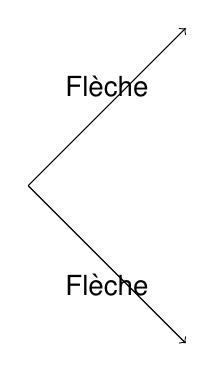
\begin{tikzpicture}
			\draw[->] (0,0) -- (2,2) node[midway, above] {Flèche};
			\draw[->] (0,0) -- (2,-2) node[midway, below] {Flèche};
		\end{tikzpicture}
	\end{block}
\end{frame}

% Section de conclusion
\section{Conclusion}

\begin{frame}{Conclusion}
	\begin{block}{Résumé}
		% Résumez les points principaux
		Résumez les points principaux de votre présentation.
	\end{block}
	\begin{alertblock}{Perspectives}
		% Proposez des perspectives
		Proposez des perspectives ou des recommandations pour l'avenir.
	\end{alertblock}
\end{frame}

% Références
\begin{frame}{Références}
	\begin{thebibliography}{9}
		\item Article 1
		\item Article 2
		\item Article 3
	\end{thebibliography}
\end{frame}

\end{document}
